% This is "sig-alternate.tex" V2.1 April 2013
% This file should be compiled with V2.5 of "sig-alternate.cls" May 2012
%
% This example file demonstrates the use of the 'sig-alternate.cls'
% V2.5 LaTeX2e document class file. It is for those submitting
% articles to ACM Conference Proceedings WHO DO NOT WISH TO
% STRICTLY ADHERE TO THE SIGS (PUBS-BOARD-ENDORSED) STYLE.
% The 'sig-alternate.cls' file will produce a similar-looking,
% albeit, 'tighter' paper resulting in, invariably, fewer pages.
%
% ----------------------------------------------------------------------------------------------------------------
% This .tex file (and associated .cls V2.5) produces:
%       1) The Permission Statement
%       2) The Conference (location) Info information
%       3) The Copyright Line with ACM data
%       4) NO page numbers
%
% as against the acm_proc_article-sp.cls file which
% DOES NOT produce 1) thru' 3) above.
%
% Using 'sig-alternate.cls' you have control, however, from within
% the source .tex file, over both the CopyrightYear
% (defaulted to 200X) and the ACM Copyright Data
% (defaulted to X-XXXXX-XX-X/XX/XX).
% e.g.
% \CopyrightYear{2007} will cause 2007 to appear in the copyright line.
% \crdata{0-12345-67-8/90/12} will cause 0-12345-67-8/90/12 to appear in the copyright line.
%
% ---------------------------------------------------------------------------------------------------------------
% This .tex source is an example which *does* use
% the .bib file (from which the .bbl file % is produced).
% REMEMBER HOWEVER: After having produced the .bbl file,
% and prior to final submission, you *NEED* to 'insert'
% your .bbl file into your source .tex file so as to provide
% ONE 'self-contained' source file.
%
% ================= IF YOU HAVE QUESTIONS =======================
% Questions regarding the SIGS styles, SIGS policies and
% procedures, Conferences etc. should be sent to
% Adrienne Griscti (griscti@acm.org)
%
% Technical questions _only_ to
% Gerald Murray (murray@hq.acm.org)
% ===============================================================
%
% For tracking purposes - this is V2.0 - May 2012

\documentclass{sig-alternate-05-2015}
\usepackage[utf8]{inputenc}

\begin{document}

% Copyright
\setcopyright{acmcopyright}
%\setcopyright{acmlicensed}
%\setcopyright{rightsretained}
%\setcopyright{usgov}
%\setcopyright{usgovmixed}
%\setcopyright{cagov}
%\setcopyright{cagovmixed}


% DOI
\doi{10.475/123_4}

% ISBN
\isbn{123-4567-24-567/08/06}

%Conference
\conferenceinfo{AsianPLoP 2016}{February 24-26, Taiwan.}

%\acmPrice{\$15.00}

%
% --- Author Metadata here ---
\conferenceinfo{WOODSTOCK}{'97 El Paso, Texas USA}
%\CopyrightYear{2007} % Allows default copyright year (20XX) to be over-ridden - IF NEED BE.
%\crdata{0-12345-67-8/90/01}  % Allows default copyright data (0-89791-88-6/97/05) to be over-ridden - IF NEED BE.
% --- End of Author Metadata ---

\title{Web Content Renderer Pattern}
%\subtitle{[Extended Abstract]
%\titlenote{A full version of this paper is available as
%\textit{Author's Guide to Preparing ACM SIG Proceedings Using
%\LaTeX$2_\epsilon$\ and BibTeX} at


\numberofauthors{3} %  in this sample file, there are a *total*
% of EIGHT authors. SIX appear on the 'first-page' (for formatting
% reasons) and the remaining two appear in the \additionalauthors section.
%

\author{
\alignauthor
Paulina Silva\\
  \affaddr{Departamento de Informática}\\
  \affaddr{Universidad Técnica Federico Santa María}\\
  \affaddr{Valparaíso, Chile}\\
  \email{pasilva@alumnos.inf.utfsm.cl}
% 2nd. author
\alignauthor
Raúl Monge\\
  \affaddr{Departamento de Informática}\\
  \affaddr{Universidad Técnica Federico Santa María}\\
  \affaddr{Valparaíso, Chile}\\
  \email{rmonge@inf.utfsm.cl}
% 3rd. author
\alignauthor 
Eduardo Fernandez\\
  \affaddr{Department of Computer \(\&\) Electrical Engineering and Computer Science}\\
  \affaddr{Florida Atlantic University}\\
  \affaddr{Florida, USA}\\
  \email{ed@cse.fau.edu}
}

\maketitle
\begin{abstract}
Currently a lot of software developments create systems that are connected to the Internet, which allows to add functionality within a system and facilities to their \textit{Stakeholders}. This leads to depend in a \textit{web client}, as the \textit{Web Browser}, which allows access to services, data or operations that the system delivers. Nevertheless, the Internet influences the attack surface of the new system, and unfortunately many stakeholders and developers are not aware of the risks they are exposed. The lack of Security Education in Software developers of a project, the low and scattered documentation of each browser (and standardization), could become a great flaw in big architectural developments which depends on the browser to do their services. A Reference Architecture of the \textit{Web Browser}, using Architectural Patterns, could be a base for understanding the security mechanisms and its architecture, which interacts with a bigger web system. This would give an unification of ideas and terminology, giving a holistic view regardless the implementation details for both the browser and the system it communicates to. We developed a Web Content Renderer Pattern which describes the infrastructure of a Renderer inside the Browser, and allows the visualization of the web content obtained in the Internet through a Web Browser. With this work we propose an Architectural Pattern as the second piece of our Reference Architecture for the Web Browser.
\end{abstract}


%
% The code below should be generated by the tool at
% http://dl.acm.org/ccs.cfm
% Please copy and paste the code instead of the example below. 
%
\begin{CCSXML}
<ccs2012>
 <concept>
  <concept_id>10010520.10010553.10010562</concept_id>
  <concept_desc>Computer systems organization~Embedded systems</concept_desc>
  <concept_significance>500</concept_significance>
 </concept>
 <concept>
  <concept_id>10010520.10010575.10010755</concept_id>
  <concept_desc>Computer systems organization~Redundancy</concept_desc>
  <concept_significance>300</concept_significance>
 </concept>
 <concept>
  <concept_id>10010520.10010553.10010554</concept_id>
  <concept_desc>Computer systems organization~Robotics</concept_desc>
  <concept_significance>100</concept_significance>
 </concept>
 <concept>
  <concept_id>10003033.10003083.10003095</concept_id>
  <concept_desc>Networks~Network reliability</concept_desc>
  <concept_significance>100</concept_significance>
 </concept>
</ccs2012>  
\end{CCSXML}

\ccsdesc[500]{Computer systems organization~Embedded systems}
\ccsdesc[300]{Computer systems organization~Redundancy}
\ccsdesc{Computer systems organization~Robotics}
\ccsdesc[100]{Networks~Network reliability}




\keywords{Web Browser, Web Client, Modular Architecture, Browser Architecture, Reference Architecture, Browser Infrastructure pattern}

\section*{Introduction}

\section*{Background}
We present in this section patterns as well as their benefits. We also describe how to build more secure reference architectures by using security patterns

Patterns are encapsulated solutions to recurrent problems and define a way to express requirements and solutions concisely, as well as providing a communication vocabulary for designers \cite{gamma1994design}. The description of architectures using patterns makes them easier to understand, provides guidelines for design and analysis, and can define a way of making their structure more secure.

Security patterns describe solutions to the problems of controlling (stopping or mitigating) a set of specific threats through some security mechanism, defined in a given context. The most common use of security patterns is to help application developers -who are not security experts- to add security in their designs. Patterns of this kind also are used to reinforce a legacy system.

The aim of a Reference Architecture is to provide a guide for developer, who are non security experts, in the development of Architectures for concrete versions of the system or to extend it. With the use of Architectural Patterns we describe the Browser Architecture as a Reference Architecture (RA). A RA is created by capturing the essentials of existing architectures and by taking into account future needs and opportunities, ranging from specific technologies, patterns and business models. It can also be derived from domain models.

A Secure Reference Architecture is a Reference Architecture where security services have been added in appropriate places to provide some degree of security for a system environment. The basic approach that we will use to build a Secure Reference Architecture is by applying a systematic methodology from [\cite{fernandez2006methodology,Fernandez2011}, which can be used as a guideline to build secure web browsers systems and/or to evaluate their security levels. We started to build a Reference Architecture as a first step, in a student work, and now we are trying to improve it using security patterns and misuse patterns. By checking if a threat, expressed as a misuse pattern, can be stopped or mitigated in the secure reference architecture, we can evaluate its level of securityx

In this work, a Browser Infrastructure Pattern is presented as a first step in to the process of developing a Secure Reference Architecture for the Web Browsr. Threat analysis and security patterns was done in our previous student work (graduation report), and we will improve it in the constrution of the SRA.

\section*{Related Work}
  \subsection*{Reference Architecture of the Browser}
  We tried to find studies by searching relevant keywords in Scopus or doing a forward snowballing from a work \cite{2005-grosskurth-browser-refarch} we knew. Unfortunately to the date there are a few works related to the construction of a Reference Architecture for the Web Browser.

  In the study made by Larrondo-Petrie et. at \cite{535061} a web browser analysis is done with the goal of obtaining a Domain Model, and Object Model and a Feature Tree which described the structure and functionality a browser had. The doamin, explained in th paper, is a distintive set of objects which 

  
  El dominio, según explica el trabajo, es un set distintivo de objetos que se comportan de acuerdo a reglas y política que caracterizan el Dominio. El Análisis de Dominio es realizado para identificar dominios y cómo éstos interactuan con otros. La metodología usada para obtener los Dominios es el \textit{Object Oriented Analyis}. Además de identificar, se clasifican estos dominios de acuerdo a su rol en el sistema terminado como: Dominio de Aplicación, Dominio de Servicio, Dominio de Arquitectura y Dominio de Implementación. El Modelo de Objetos sirve para entregar más detalles, un resumen general de las Entidades del \textit{Web Browser} y sus relaciones. El \textit{Feature Tree} pretende entregar detalles sobre los aspectos funcionales de la aplicación. El Modelo planteado, śegún el artículo, debería ser útil para los Desarrolladores de Software que construyen \textbf{Aplicaciones Web basadas en el uso del \textit{Browser}}.  Este estudio se encuentra bastante lejos de lo que se quiere hacer en este trabajo, pero sirve para obtener un transfondo de lo que sucede en el \textit{\textit{Web Browser}}, aún cuando la información esté muy desactualizada.

  En el trabajo de Grosskurth et al. \cite{2005-grosskurth-browser-refarch, preprint-grosskurth-browser-archevol} se utiliza una herramienta de ingeniería inversa, para obtener una arquitectura de referencia de muy alto nivel en base a dos navegadores open-source: Mozilla y Konqueror. Lo obtenido captura los subsistemas fundamentales comunes a los sistemas del mismo dominio, así como las relaciones entre estos subsistemas. En esta arquitectura se identifican los siguientes subcomponentes: Interfaz Usuaria, Persistencia de Datos, Browser Engine, Rendering Engine, Networking, Interprete de Javascript, XML Parser y Display Backend. Se menciona que estos componentes están estrechamente integrados (high coupling) con el Rendering Engine, lo cual tiene sentido en la arquitectura monoproceso que poseen Mozilla y Konqueror; es una decisión de diseño muy común en los \textit{Browser} de la época. Al identificar estos componentes, se comenta que esto podría servir tanto en el diseño y durante la mantención de un sistema, pues mejora el entendimiento de ésta al ayudar a analizar los trade-off entre diferentes opciones de diseño; o también puede servir como un \textit{template} para obtener nuevos diseños. Una vez obtenida la arquitectura conceptual, se inició una evaluación de ésta al comparar las arquitecturas concretas de cada browser open-source, extraídas desde el código fuente, para ver qué tanto el modelo conceptual era cercano a la realidad; la constante comparación permitió ademas refinar la Arquitectura de Referencia. Los browsers usados para validar fueron: Epiphany, Safari, Lynx, Mosaic y Firefox. Si bien la arquitectura presentada entrega bastante información a alto nivel, no desarrolla más que esa capa de abstracción, además parece ser que depende también de la implementación usada en la herramienta de ingeniería inversa. 

  En el documento \cite{Godfrey2000} realizado en el año 2000, se describe la experiencia realizada al extender el trabajo del proyecto TAXFORM. Usando PBS, una herramienta de Ingeniería Inversa, se extrajo la arquitectura de software del navegador Mozilla, con el objetivo de entender la estructuración de sus componentes; además de crear vistas arquitecturales de alto nivel del sistema. El modelo arquitectónico obtenido contiene 11 subsistemas de alto nivel, de éstos los que más se destacaron fue el \textit{HTML Layout}, la implementación de herramientas y el código de la interfaz de usuario. En el año en que se lleva a cabo este estudio (2000), se menciona que la arquitectura ha decaído significativamente en muy poco tiempo, o su arquitectura no fue planificada cuidadosamente desde el comienzo; parte de lo anterior, el autor cree que es secuela de la \textit{Guerra de Navegadores}. Si bien el trabajo ayuda a entender un poco la estructura detrás del navegador, este trabajo es muy antiguo y la versión más actual del navegador ha cambiado bastante. Además, lamentablemente el enfoque de este estudio no es intentar entender lo que hace cada subsistema, si no que es la implementación de la herramienta misma para obtener la arquitectura de software del browser seleccionado.

  %Lwin2009 - Agent Based Web Browser
  En \cite{Lwin2009} se propone un \textit{Browser} llamado Anfel SOFT, donde gracias al uso de Inteligencia Artificial, crea agentes que permiten mejorar la experiencia del usuario. El trabajo asegura que el browser será capaz de aprender el comportamiento de navegación del usuario, y guiará al usuario en su navegación para que ésta sea lo más efectiva posible. El paper obtiene los subsistemas que se pueden encontrar en un browser de la misma manera que lo realiza \cite{2005-grosskurth-browser-refarch}. Si bien la arquitectura que muestra refleja parte de lo visto en los 3 browsers escogidos en este estudio, no da detalles acerca de cada subsistema identificado. Además la Arquitectura de Referencia que entrega es la misma vista en \cite{2005-grosskurth-browser-refarch, preprint-grosskurth-browser-archevol}, y a pesar que identifica otros posibles componentes, no agrega nada nuevo.

  Podemos ver en los trabajos que algunos construyen una Arquitectura de Referencia basada en técnicas de Ingeniería Inversa. En cada uno de ellos el trabajo ha sido a muy alto nivel y la descripción de los subcomponetes del sistema es mínima. Si bien explican las relaciones entre éstos, no dan un mayor entendimiento en cómo se comportan en ciertas situaciones. En este trabajo se espera profundizar un poco más en la abstracción obtenida, incluyendo información de tanto los casos de uso del \textit{Browser} como las actividades que se realizan con otros usuarios. Desafortunadamente para esta memoria, no existe mucha literatura sobre el desarrollo de una Arquitectura de Referencia del \textit{Browser}, y de lo que hay, el trabajo más actual es el realizado por \cite{Lwin2009} en el año 2009.

  \subsection*{Secure Software Development}
  La literatura que habla de la construcción de \textit{Secure Software} o Software Seguro, indica que los practicantes de Desarrollo de Software deben entender, en gran medida, los problemas de seguridad que podrían llegar a ocurrir en sus sistemas. No basta con saber cómo unir las piezas, no basta con que cada pieza de por si sea segura, si los componentes del sistema no actuan de forma coordinada, probablemente éste no será seguro \cite{fernandez2013security}, dado que la seguridad es una Propiedad Sistémica que necesita ser vista de manera holística y al inicio del proceso.



\section*{Browser Infrastructure Pattern}

  \subsection*{Intent}
  The Browser Infrastructure Pattern allows the request of a web resource in the Internet to a \textbf{Browser User} (BU), which is a user who uses a Browser within a \textbf{Host}. The Pattern lets visualize the communication between the components that make the Web Browser and the Provider (i.e, a Server), to whom the request is made.

  \subsection*{Example}
  Within the Host it is possible a lack of resources that a Host user may need. The request of external services or resources is the main reason of the Internet existence. This kind of task it is possible to do in a lot of ways, it all depends on what the Provider wish to deliver to others.
  
  \subsection*{Context}
  Browser User is a Host user which uses a Browser, and the Provider is an entity which can be accessed in the Internet. The contact between each other is normally done by Web Applications or Servers which communicats using the HTTP protocol. A Browser let the Browser User access and visualize the external resources a Provider has and a Browser User may need.
  
  \subsection*{Problem}
  Some Browser Users could need resources from a Providr, but the user maybe will need them in a special format o they should be presented in the screen of the computer to be visualized. In this case, if an appropiate tools is not used, the resource could not be helpful if it can not be used correctly. How can the Host and Provider be prepared to this situation? The solution to this problem must resolve the following problems:
  \begin{itemize}
    \item Transparency: the user behind the Host should not be worried of what it is done, while a request to a Provider has been issued. 
    \item Stability: The \textit{Browser} must be capable of working, evn if a web page had a problem to be seen or there is an internal problem.
    \item Isolation: Each \textit{request} must not interrupt others.
    \item Heterogeneity: It does not matter the type of Provider to which the Browser communicats, it should be possible to interact with whatever type is it, and also it should be capable to show adequately the content of the obtained resource.
    \item Availability: The user of the Host, should be capable to requst at any time.
  \end{itemize}

  \subsection*{Solution}
  Un \textit{Web Browser} puede satisfacer las \textit{request} del user del Host a traés de un Browser User, ya sea por una o varias instancias de Browser User, lo que permite tener una diversidad de opciones para navegar por sitios de Internet. Un \textit{Browser} debe ser capaz de poder entregar una navegación rápida y estable, sin que cada sitio accedido afecte a los otros recursos adquiridos.

    \subsubsection*{Structure}
    El Browser Client (BC) es la entidad que representa el proceso principal de un navegador Web y comprende la cantidad mínima de componentes que constituye un \textit{Web Browser}. Un Host (H) que aloja e interactua con el BC, está compuesto por Hardware (HW) y un Sistema Operativo (SO). Al mismo tiempo, el Provider (P) posee también HW y SO, pero adicionalmente posee un Web Server (WS) que se encarga de recibir las peticiones externas. Browser Client, Sandbox, GPU Instance (GPUI) y Plugin son del tipo Process (Pr), que residen dentro de un Host (H) con un cierto tipo de sistema Operativo (OS). La mayoría de los navegadores existentes usan un componente central para realizar las operaciones que necesitan afectar al Host del \textit{Browser}. La figura \ref{fig:BIPatt} muestra el diagrama del clases para el patrón Browser Infrastructure. Por cada recurso que un BC solicite, se crearán Sandbox (S) que alojarán una instancia del patrón Web Content Renderer el que permiten realizar la navegación y posterior visualización del recurso.
    El componente BC actúa como un broker de las solicitudes de las Sandbox, lo que permite tener un control fino de los mensajes enviados, usando IPC/IPDL/COM, entre los procesos que se comunican. El GPU Instance y Plugins son elementos que pueden comunicarse directamente con el Sandbox, de esta manera cualquier necesidad de recursos del Host pasarán también por el Browser Client. 
    Un usuario que desee hacer un \textit{request} de un recurso en Internet por medio de un navegador es lo que llamaremos Browser User (BU). Éste usa el Browser Client para realizar peticiones al Provider, donde éste último posiblemente utilice un Web Server para ese cometido (Figura \ref{fig:BIPatt})
    \begin{figure*}[h!t]
      \centering
      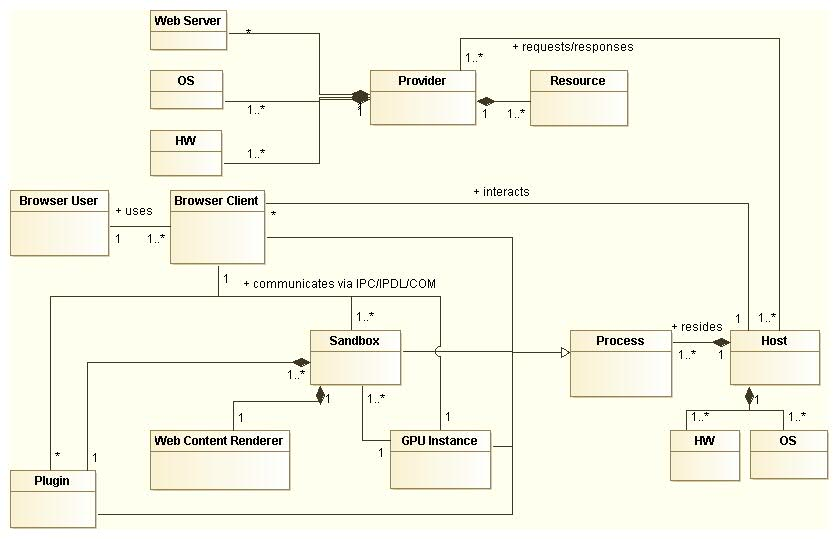
\includegraphics[scale=0.55]{figures/browserInfraPattern_v3.jpg}
      \caption{Componentes de alto nivel del \textit{Browser}.}
      \label{fig:BIPatt}
    \end{figure*}

    \subsubsection*{Dynamics}
    Los casos de uso relacionados al patrón son los siguientes:
    \begin{itemize}
      \item Realizar request (actor: Browser User)
      \item Cancelar request (actor: Browser User)
      \item Guardar recurso (actor: Browser User)
      \item Recibir Request (actor: Provider)
      \item Pedir recursos (actor: Host)
    \end{itemize}
    Detallaremos el caso de uso Realizar Request (Figura \ref{fig:SecReq}):
    \subsubsection*{Sumario} Un Browser User requiere de abrir un recurso URL que puede ser obtenido mediante el uso del protocolo HTTP, según los requerimientos del Provider. El Browser Client será usado por un Browser User para poder realizar la visualización del recurso URL.
    \subsubsection*{Actor} Browser User
    \subsubsection*{Precondiciones} El Host debe tener uno o más Browser Client para el usuario del Host. Además de estar conectado a una red o Internet. El Provider al que se desea contactar también debe estar disponible.
    \subsubsection*{Descripción}
    Nota: Los mensajes entre el Browser Client y el Sandbox pueden ser tanto síncronos como asíncronos \cite{firefoxIPC,GCIPC}. No especificaremos en gran detalle , pues lo que importa en este trabajo será el origen y destino de los mensajes (no está dentro del ámbito ver la sincronización).
      \begin{enumerate}
        \item Un Browser User requiere acceder a una URL para obtener cierto recurso de un Provider, para esto usa un Browser Client ya instanciado por el Host. En el interior del Sandbox existe una instancia del patrón Web Content Renderer. 
        \item El Sandbox requiere los recursos del Host para obtener lo que hay detrás de la URL. Una petición es realizada desde el Sandbox al Browser Client a través de un canal de comunicación como: IPC, IPDL o COM (dependiendo el tipo de \textit{Browser} usado), usando la API limitada que posee para comunicarse a un proceso de mayor privilegio. 
        \item El Browser Client recibe la solicitud, verifica a través de su motor de políticas/normas si la acción del Sandbox puede ser permitida.
        \item Si es permitada la acción del Sandbox, se utilizará la Network API que contiene el Browser Client para obtener recursos del Host (a través de llamadas al sistema). El Browser Client se comunica internamente con el Host, y este último debe revisar sus políticas y asegurarse que el Browser Client posee el privilegio de hacer la petición del recurso del Host.
        \item Si se permite el acceso el recurso, el Browser Client podrá realizar un \textit{request} a través de la Network API. Si el \textit{request} no es del tipo \textit{pre-flight}, el Provider recibirá el \textit{request} y trabajará sobre la petición.
        \item El Provider enviará un \textit{response} al \textit{request} enviado. Dependiendo como esté implementado el Browser Client, éste podría o no tener que esperar a la respuesta (síncrono o asíncrono) del Provider.
        \item Una vez obtenida la respuesta ésta es almacenada en cache, salvo que indique de no hacerlo.
        \item La respuesta del \textit{request} es enviada por el canal de comunicación al Sandbox del que se originó y posteriormente al Web Content Renderer. Si fue recibida una respuesta por parte de la \textit{request}, el Web Content Renderer está listo para preparar el parsing de la página web o utiliza un plugin o GPU para apoyar la visualización del recurso obtenido por la URL. En caso contrario el Web Content Renderer dentro del Sandbox creará una página de error.
        \item El \textit{Renderer} obtiene un bitmap que debe enviar al Browser Client, para que el Host pueda mostrarlo visualmente. Antes de realizarlo, debe revisar que el Sandbox que contiene el Web Content Renderer posea los permisos.
        \item Si los permisos son suficientes, el Browser Client envía el bitmap como parámetro en la llamada al sistema realizada al Host. Finalmente, el Host debe revisar que la llamada al sistema que realizó el Browser Client, tenga los permisos necesarios; de poseerlos, el bitmap se mostrará al Browser User por pantalla.
      \end{enumerate}
    \subsubsection*{Curso Alternativo} 
    \begin{itemize}
    \item El Provider no esté disponible.
    \item El recurso al que apunta la URL no exista.
    \item Se cancela el \textit{request} realizado.
      \end{itemize}
    \subsubsection*{Condiciones póstumas} El \textit{Browser} recibe el recurso indicado por la URL y se muestra por el perísférico la salida del recurso al usuario del Host.
      \begin{figure*}[h!t]
          \centering
          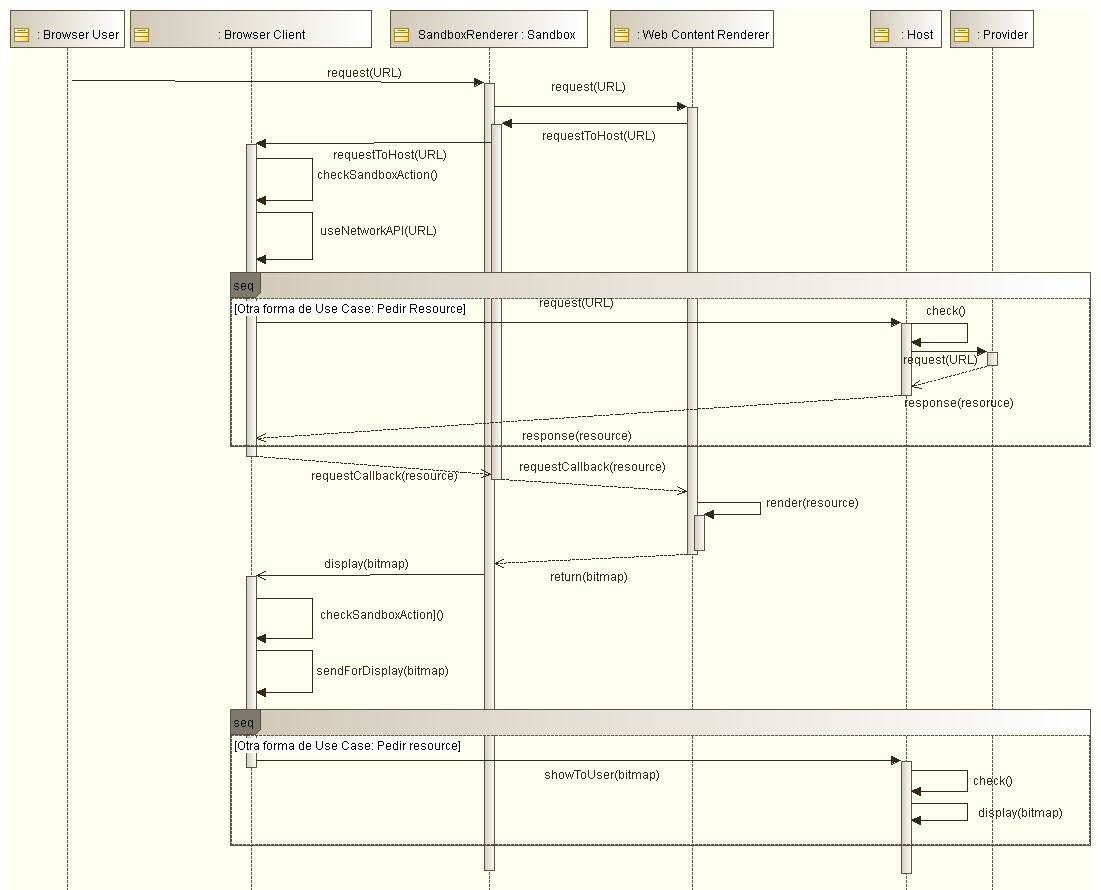
\includegraphics[scale=0.61]{figures/requestResource_v2.jpg}
          \caption{Diagrama de Secuencia: Realizar Request.}
          \label{fig:SecReq}
      \end{figure*}

  \subsection*{Implementation}
  \begin{itemize}
    \item El Sandbox puede ser implementado de diversas maneras. Google Chrome \cite{sandboxGC} se basa en no reinventar la rueda y utiliza los mecanismos de protección que el Sistema Operativo (por ejemplo: Windows o Linux) del Host ya tiene incorporados para proteger al usuario, evitando que el proceso no tenga acceso al sistema de archivos y teniendo una API de llamadas al sistema muy restrictivas en el Web Content Renderer. Google Chrome, Firefox e Internet Explorer asumen que los Sandoboxs son procesos que deben regirse bajo el principio de menor privilegio (least privilege). La mínima configuración del Sandbox se compone de 2 procesos: El proceso privilegiado o Broker que es representado por el Browser Client, y el o los procesos que están bajo el Sandbox o targets.
    \item Para hacer cumplir con el Same Origin Policy, Google Chrome, Firefox e Internet Explorer utilizan diferentes esquemas; por ejemplo: Google Chrome deja el trabajo a su Renderer (Web Content Renderer en este caso) para dejar aisladas las páginas/recursos de diversos sitios.
  \end{itemize}

  \subsection*{Consequences}
  El patrón Browser Infrastructure provee los siguientes beneficios:
  \begin{itemize}
    \item Transparencia: La navegación del usuario se realizará casi de manera automática, solo en casos muy puntuales el usuario tendrá que tomar una decisión sobre el recurso que desea pedir.
    \item Estabilidad: Gracias a que el Browser Client, Sandbox, Plugin y GPU Instance son procesos del Host independientes, el fallo de uno no generará problemas en el otro (crash, corrupción de memoria, etc).
    \item Aislación: Dependiendo del tipo de aislación es posible separar los distintas peticiones, de manera que no interfieran entre sí, a menos que se desee.
    \item Heterogeneidad: Dado que cada Browser Client trata de seguir los estándares de la W3C, toda página que también siga éstas guías podrá ser visualizada, así como también otro tipo de recursos.
    \item Disponibilidad: Cada proceso es independiente y posee sus propias hebras de ejecución, y fueron creadas específicamente para que la interfaz de usuario pueda mantenerse fluida.
  \end{itemize}
  Al mismo tiempo, el patrón posee las siguientes debilidades:
  \begin{itemize}
    \item Dado que se inician procesos independientes para navegar a un recurso (dependiendo el esquema que utilice el browser), es posible que una gran cantidad de recursos se vayan a usar para mantener todo abierto.
    \item Aquellos Provider que no hayan cumplido con las especificaciones de la W3C, mostrarán su resource de forma incorrecta por el \textit{Web Browser}.
  \end{itemize}

  \subsection*{Example Resolved}
  Con el patrón entregado ahora es posible poder navegar de forma fluida a todos los recursos en la Internet que deseamos. Es posible proveer a través de la aislación de los componentes: rapidez, seguridad y estabilidad. El Browser User solamente se molestará en la navegación, cuando se requiera de su autorización para ingresar a ciertos recursos del Host que sean privilegiados, como el sistema de archivos. Cada usuario del Host, puede utilizar el Browser Client que desee, dado que cada uno de ellos es aislado por procesos independientes, así también los otros Browser Clients entre si.

  \subsection*{Known Uses}
  \begin{itemize}
    \item Actualmente, la separación de los componentes del \textit{Browser} en varios procesos, con diferentes niveles de acceso, se conoce como una Arquitectura Modular \cite{Vrbanec2013}. Esto permite la separación de preocupaciones del navegador, lo que se traduce en una mayor estabilidad, aislación, seguridad y rapidez.
    \item Google Chrome se basa en la arquitectura modular, donde cada proceso Renderer se comunica con el Browser Kernel \cite{multiProcGC}. Internet Explorer, por ser privativo no da mucha información sobre su estructura o detalles de su implementación; \cite{Crowley2010} sobre la arquitectura Loosely-Coupled \cite{IE8-LCIE} y sus componentes, pero sin entrar tanto en detalle. Firefox, por su parte posee las dos implementaciones: monoprocesos y multiproceso. Electrolysis es el nombre de la arquitectura modular que se está implementado, pero que aún no ha sido finalizada completamente.
  \end{itemize}

  \subsection*{Related Patterns}
  \begin{itemize}
    \item El patrón Web Content Renderer, el cuál está en proceso de desarrollo, representa el subsistema dentro del Sandbox que permite realizar el parsing del \textit{resource} o recurso obtenido por medio de una petición.
    \item El patrón Browser Kernel, también en desarrollo, representa el subsistema que representa el navegador Web. Este componente actua como un Reference Monitor \cite{fernandez2013security} para todas las solicitudes que el Renderer llegara a necesitar.
    \item El Sandbox se comunica con el Browser Client siguiendo un patrón como el que indica el Policy Authorization \cite{fernandez2013security}. Por cada petición del Renderer, el Sandbox tendrá el acceso si las políticas que el Browser Client permiten tal acción.
  \end{itemize}

\section*{Conclusions}
Un navegador Web pareciera ser un Software de mediana complejidad para tanto usuarios como desarrolladores sin experiencia en seguridad, pero lamentablemente esta pieza de Software permite realizar una variadad de vectores de ataque, tanto en un usuario usándolo como en el sistema con el que interactúa. Por lo tanto es importante comprender su estructura y como éste interactúa con Stakeholders internos como externos.

Es de esperarse que en el futuro la mayoría de los \textit{Web Browser} tomen forma de una Arquitectura Modular. Por lo tanto, es importante que los desarrolladores conozcan los procesos internos del \textit{Web Browser} al momento de desarrollar un sistema que se comunicará con éste. Tanto la Arquitectura de Referencia como el patrón de Mal Uso presentados, apuntan a entregar el conocimiento básico de los componentes e interacciones entre el \textit{Web Browser} y un proveedor de recursos externo; así como también de las amenazas que existen.

Construcción del primer Patrón Arquitectural sobre la infraestructura del \textit{Web Browser}, para poder entender de manera holística los componentes, interacciones y relaciones. Una parte de la Arquitectura de Referencia ha sido construída, a través de la abstracción del Patrón Browser Infrastructure. Además se ha conseguido caracterizar los Stakeholders y uno de los caso de uso más importantes. De lo que tenemos por conocido, esta es la segunda Arquitectura de Referencia construída del \textit{Browser}. 

El trabajo propuesto permite comprender mejor, por medio de la Arquitectura de Referencia parcialmente construída, tanto componentes como amenazas existentes. Además como no está sujeto a implementaciones específicas, es posible generalizar ciertos resultados en otros Browsers.


\section*{Future Work}
El trabajo futuro que se realizará para obtener el grado de Magister, irá relacionado a la creación de una Arquitectura de Referencia de seguridad del \textit{Web Browser}, utilizando la misma metodología presentada acá. Otros patrones relacionados al Patrón Browser Infrastructure serán obtenidos para así completar la AR ya iniciada, como por ejemplo el patrón Web Content Renderer y Browser Kernel. Un ejemplo del tipo de trabajo que se pretende realizar puede ser vista en \cite{fernandez2014security}, donde este estudio realiza actividades para poder construir software seguro y evaluar los niveles de seguridad de un sistema ya construído.

Se planea construir más Patrones de Mal Uso, para el Patrón Browser Infrastructure para continuar con el estudio de amenazas posibles dentro del \textit{Browser}, como una manera de educar a los Desarrolladores y Stakeholders de los peligros existentes. Al mismo tiempo estos patrones permitirán la construcción de esta AR de seguridad. En esta misma dirección, además de encontrar las amenazas posibles de existir en el sistema, se necesita encontrar las contramedidas o defensas de seguridad que permitan evitar o preveer esas amenazas a través de Patrones de Seguridad sobre la Arquitectura de Referencia construída. Lo anterior es posible de realizar bajo el mismo ejercicio ya realizado en este trabajo, buscando amenazas sobre cada acción realizada en cada Caso de Uso del navegador.

En cuanto a los \textit{Web Browser}, los ataques basados en Ingeniería Social parece que no disminuirán en un buen tiempo, pues no existen tecnologías actuales que puedan detectar en un \(100\%\) y sin falsos positivos los posibles peligros que pueden traer. Tecnologías como CAMP (Content-Agnostic Malware Protection) parecen ser parte de la solución, pero aún están lejos de ser perfectos.

%ACKNOWLEDGMENTS are optional
%\section{Acknowledgments}


\bibliographystyle{abbrv}
\bibliography{refTodas}  


\end{document}
